
\chapter{Classical Density Functional Theory\label{chpt:mdft}}

Classical density functional theory (DFT) provides a framework for determining
thermodynamic properties and correlation functions over a wide variety
of inhomogeneous (model) fluids beginning from a microscopic basis,
i.e. the Hamiltonian describing interactions between particles. DFT
is based on the principle that the grand potential of a specified inhomogeneous
fluid is a functional of the average one-body density,

\[
\rho(r)=\left\langle \sum_{i=1}^{N}\delta(\mathbf{r}-\mathbf{r}_{i})\right\rangle 
\]
where $\mathbf{r_{i}}$ is the position coordinate of particle $i$.

This article describes all the fundamental theories behind different Molecular Density Functional Theory (MDFT) 
algorithms involved in this thesis to evaluate excess free energy
functional $\mathcal{F}_{\mathrm{exc}}$ under HRF approximation.


\section{Equilibrium Classical DFT}


\section{Variation principle}

The key idea is that $\mathcal{F}[\rho]$ is a unique functional of
$\rho(\mathbf{r})$; its form does not depend on the external potential
$V(\mathbf{r})$. \textcolor{red}{!!!!}

variation principle: pair minimization

In \acf{MDFT}, the grand potential density functional corresponding
to an inhomogeneous fluid density $\rho(\mathbf{r},\mathbf{\Omega})$
is given by 
\begin{equation}
\Theta[\rho(\mathbf{r},\mathbf{\Omega})]=\Theta[\rho_{0}]+\mathcal{F}[\rho(\mathbf{r},\mathbf{\Omega})]
\end{equation}
where $\Theta[\rho_{0}]$ is the correspondent reference bulk fluid
grand potential and $\rho$ is the fluid density function variable
of 3 to 6 dimensions, including 3 coordinations for the position part,
and 0 to 3 for the angular part. For instance, in an isotropic fluid: 

\begin{equation}
\rho(\mathbf{r},\mathbf{\Omega})=\left\{ \begin{array}{ll}
n(\mathbf{r}) & \mbox{if atomic, }\Omega\equiv1\\
n(\mathbf{r})/4\pi & \mbox{if linear, }\Omega\equiv(\theta,\phi)\\
n(\mathbf{r})/8\pi^{2} & \mbox{if non-linear, }\Omega\equiv(\theta,\phi,\psi)
\end{array}\right.\label{eq:rho}
\end{equation}


Here the $4\pi$ and $8\pi^{2}$ is the normalization factor which equals
to $\int\mathrm{d}\mathbf{\Omega}$. The 6D definition of the latest
case in eq. \ref{eq:rho} of $\rho(\mathbf{r},\mathbf{\Omega})$ is
needed for arbitrary solvents, which results in the most complex form
of the functional. 

According to the variation principle (c.f. Evans), the equilibrium
density can be found by minimizing the free energy functional $\mathcal{F}[\rho]$
regarding $\rho(\mathbf{r},\mathbf{\Omega})$: 
\begin{equation}
\frac{\delta\mathcal{F}[\rho]}{\delta\rho(\mathbf{r},\mathbf{\Omega})}|_{\rho=\rho_{0}}=0
\end{equation}


And this functional is defined as a sum of functional contributions: 

\begin{equation}
\mathcal{F}[\rho]=\mathcal{F}_{\mathrm{id}}[\rho]+\mathcal{F}_{\mathrm{ext}}[\rho]+\mathcal{F}_{\mathrm{exc}}[\rho]
\end{equation}


The ideal term $\mathcal{F}_{\mathrm{id}}[\rho]$ is deduced from
the particle interaction-free condition: 
\begin{equation}
\mathcal{F}_{\mathrm{id}}[\rho]=\beta^{-1}\int\mathrm{d}\mathbf{r}\mathrm{d\Omega}\left[\mathbf{\mathbf{\ln\left(\frac{\rho(\mathbf{r},\mathbf{\mathbf{\mathbf{\mathbf{\Omega}}}})}{\rho_{0}}\right)}}-\rho(\mathbf{r},\mathbf{\mathbf{\mathbf{\Omega}}})+\rho_{0}\right]
\end{equation}
where $\beta=\left(K_{\mathrm{B}}T\right)^{-1}$ and $\rho_{0}$ are
the reference bulk density of pure solvents. 

The external potential term calculates the contribution of solute
external potential $V_{\mathrm{ext}}$: 
\begin{equation}
\mathcal{F}_{\mathrm{ext}}[\rho]=\int\mathrm{d}\mathbf{r}\mathrm{d}\mathbf{\mathbf{\Omega}}V_{\mathrm{ext}}(\mathbf{r},\mathbf{\mathbf{\mathbf{\mathbf{\Omega}}}})\rho(\mathbf{r},\mathbf{\mathbf{\mathbf{\mathbf{\Omega}}}})
\end{equation}


\begin{equation}
V_{\mathrm{ext}}(\mathbf{r},\mathbf{\mathbf{\mathbf{\mathbf{\Omega}}}})=\sum_{j\in\mathrm{solvent}}\left\{ q_{j}V_{q}(\mathbf{r}_{j})+\sum_{i\in\mathrm{solute}}4\epsilon_{ij}\left[\left(\frac{\sigma_{ij}}{r_{ij}}\right)^{12}-\left(\frac{\sigma_{ij}}{r_{ij}}\right)^{6}\right]\right\} 
\end{equation}
where $V_{\mathrm{ext}}$ is pre-calculated and stored as a 6-dimension
double precision (8 bytes per real value) table. It contains the contribution
of Lennard-Jones interaction and electrostatic potential. 

These two terms, $\mathcal{F}_{\mathrm{id}}[\rho]$ and $\mathcal{F}_{\mathrm{ext}}[\rho]$,
are physically exact. 

The excess term $\mathcal{F}_{\mathrm{exc}}[\rho]$ depends on the
exact correlation function, which is a priori unknown: 
\begin{equation}
C(\mathbf{r}_{1},\mathbf{r}_{2},\mathbf{\Omega}_{1},\mathbf{\Omega}_{2};\rho)\equiv\frac{\beta\delta^{2}\mathcal{F}_{\mathrm{exc}}[\rho]}{\delta\rho(\mathbf{r}_{1},\mathbf{\Omega}_{1})\delta\rho(\mathbf{r}_{2},\mathbf{\Omega}_{2})}
\end{equation}


The ideal term $\mathcal{F}_{id}[\rho]$ is deduced from the condition
that the interaction potential of particles is $\Phi=0$ 
\[
Z_{N}(\beta,V)=\frac{\lambda^{-3N}}{N!}\int_{V}d\mathbf{r}^{N}e^{-\beta\Phi}=\frac{\lambda^{-3N}}{N!}V^{N}
\]
\[
F_{N}(\beta,V)=-\beta^{-1}\log{Z_{N}}=\beta^{-1}\log{(N!\lambda^{3N}V^{-N})}=\beta^{-1}(N\log{\lambda^{3}\rho}-N)
\]


(also available for the inhomogenous case.) Since we define 
\[
\mathcal{F}_{id}[\rho]=\int d\mathbf{X}f_{id}[\rho(\mathbf{X})]
\]
we have 
\[
f_{id}[\rho(\mathbf{X})]=\beta^{-1}\Delta\rho(\log{\lambda^{3}\Delta\rho}-1)
\]
and 
\[
\mathcal{F}_{id}[\rho]=\beta^{-1}\int d\mathbf{X}_{1}[\rho(\mathbf{X}_{1})\log{(\frac{\rho(\mathbf{X}_{1})}{\rho_{0}})}-\rho(\mathbf{X}_{1})+\rho_{0}]
\]


The external potential term is
\[
\mathcal{F}_{ext}[\rho]=\int d\mathbf{X}_{1}V_{ext}(\mathbf{X}_{1})\rho(\mathbf{X}_{1})
\]
where $V_{ext}$ is given by table.

The exact (in an approximation where C does not depend on $\rho$) form
of the excess term $\mathcal{F}_{exc}$ is 
\[
\mathcal{F}_{exc}[\rho]=\beta^{-1}\int d\mathbf{X}_{1}d\mathbf{X}_{2}\Delta\rho(\mathbf{X}_{1})\Delta\rho(\mathbf{X}_{2})C(\mathbf{X}_{1},\mathbf{X}_{2};\rho)
\]


where $C(\mathbf{X}_{1},\mathbf{X}_{2};\rho)$ is the correlation
function, a priori unknown, the definition of which is: 
\[
C(\mathbf{X}_{1},\mathbf{X}_{2};\rho)=\frac{\beta\delta^{2}\mathcal{F}_{exc}[\rho]}{\delta\rho(\mathbf{r}_{1})\delta\rho(\mathbf{r}_{2})}
\]


Structure MDFT

The code MDFT is built for minimizing the free energy functional $\mathcal{F}[\rho]$
by minimizer L-BFGS (ref). Its main structure is shown in fig. 

\begin{figure}[h]
\caption{\selectlanguage{english}%
Flowchart of code MDFT\selectlanguage{american}%
}
\end{figure}


The minimizer requires the functional and its gradient as input, and
at each iteration produces a new fluid density $\text{\ensuremath{\rho}(\ensuremath{\mathbf{r}},\ensuremath{\mathbf{\mathbf{\mathbf{\Omega}}}})}$
closer to the equilibrium density. The objective for \textbf{branch
hesper} is to calculate the excess term $\mathcal{F}_{\mathrm{exc}}[\rho]$
of the functional in eq.\ref{eq:F_exc}, as well as its gradient: 

\begin{equation}
\gamma(\mathbf{r}_{1},\mathbf{\Omega})=\frac{\delta\mathcal{F}_{\mathrm{exc}}}{\delta\rho}=-\beta^{-1}\int d\mathbf{r}_{2}d\mathbf{\Omega}_{2}\Delta\rho(\mathbf{r}_{2},\mathbf{\Omega}_{2})c^{(2)}(\mathbf{r}_{12},\mathbf{\Omega}_{1},\mathbf{\Omega}_{2})\label{eq:gradient}
\end{equation}



\section{Ideal free energy}


\section{External free energy}


\subsection{Electrostatic potential}

The direct evaluation of the Coulomb sum for $N$ particles is 
\begin{equation}
U_{C}=\sum_{i<j}a\frac{q_{i}q_{j}}{\left\Vert \bm{r}_{i}-\bm{r}_{j}\right\Vert },\label{eq:direct-coulomb-sum}
\end{equation}
where $a$ is a constant that gives $U_{C}$ the dimension of an energy,
and $q_{i}$,$\bm{r}_{i}$ are the charge and position of particle
$i$. The computation of equation \ref{eq:direct-coulomb-sum} is
demanding because it requires a large number of distances $r_{ij}\equiv\left\Vert \bm{r}_{i}-\bm{r}_{j}\right\Vert $
to be computed. In our case, we have $\textrm{nfft}_{1}\times\textrm{nfft}_{2}\times\textrm{nfft}_{3}\times N_{\bm{\Omega}}\times N_{\psi}\times N_{q_{v}}$,
where $N_{q_{v}}$ is the number of point charges of the solvent molecule
to be computed per point charge of the solute. This is typically $10^{9}$
distances for MDFT.

L'énergie électrostatique s'écrit
\begin{eqnarray}
\mathcal{F}_{q} & = & \frac{1}{2}\iiint\frac{\rho_{c}^{\textrm{soluté}}\left(\boldsymbol{r^{\prime}}\right)\rho_{c}^{\textrm{solvant}}\left(\boldsymbol{r},\boldsymbol{\Omega}\right)}{4\pi\epsilon_{0}\left\Vert \boldsymbol{r}-\boldsymbol{r^{\prime}}\right\Vert }\textrm{d}\boldsymbol{r}\textrm{d}\boldsymbol{r^{\prime}}\textrm{d}\boldsymbol{\Omega}\\
 & = & \frac{1}{2}\frac{1}{4\pi\epsilon_{0}}\iiint\frac{\rho_{c}^{\textrm{soluté}}\left(\boldsymbol{r^{\prime}}\right)}{\left\Vert \boldsymbol{r}-\boldsymbol{r^{\prime}}\right\Vert }\left[\rho^{\textrm{solvant}}*\sigma\right]\left(\boldsymbol{r},\boldsymbol{\Omega}\right)\textrm{d}\boldsymbol{r}\textrm{d}\boldsymbol{r^{\prime}}\textrm{d}\boldsymbol{\Omega}\\
 & = & \frac{1}{2}\frac{1}{4\pi\epsilon_{0}}\iint\left[\rho_{c}^{\textrm{soluté}}*\left\Vert \boldsymbol{r}\right\Vert ^{-1}\right]\left(\boldsymbol{r},\boldsymbol{\Omega}\right)\left[\rho^{\textrm{solvant}}*\sigma\right]\left(\boldsymbol{r},\boldsymbol{\Omega}\right)\textrm{d}\boldsymbol{r}\textrm{d}\boldsymbol{\Omega}\\
 & =
\end{eqnarray}


On définit une densité de charge d'une molécule $\boldsymbol{\sigma}\left(\boldsymbol{r},\boldsymbol{\Omega}\right)$:
\begin{equation}
\boldsymbol{\sigma}\left(\boldsymbol{r},\boldsymbol{\Omega}\right)=\sum_{m=1}^{\textrm{sites du solvant}}q_{m}\delta\left(\boldsymbol{r}-\boldsymbol{s}_{m}\left(\boldsymbol{\Omega}\right)\right).
\end{equation}
$\boldsymbol{s}_{m}\left(\boldsymbol{\Omega}\right)$ désigne la position
du $m^{\textrm{ième}}$ site de la molécule de solvant quand elle
a l'orientation $\boldsymbol{\Omega}$.


\section{Excess free energy}

In the molecular density functional theory (MDFT), the excess free
energy functional $\mathcal{F}_{\mathrm{exc}}$ can be developed via
Taylor expansion: 
\begin{equation}
\mathcal{F}_{\mathrm{exc}}\left[\rho\right]\equiv\mathcal{F}_{\mathrm{exc}}\left[\rho_{0}\right]+\int\mathrm{d}\mathbf{X_{1}}\frac{\delta\mathcal{F}_{\mathrm{exc}}\left[\rho\right]}{\mathrm{\delta}\rho(\mathbf{X_{1}})}\Delta\rho(\mathbf{X_{1}})+\frac{1}{2}\int\mathrm{d}\mathbf{X_{1}}\mathrm{d}\mathbf{X_{2}}\frac{\mathrm{\delta}^{2}\mathcal{F}_{\mathrm{exc}}\left[\rho\right]}{\mathrm{\delta}\rho(\mathbf{X_{1}})\mathrm{\delta}\rho(\mathbf{X_{2}})}\Delta\rho(\mathbf{X_{1}})\Delta\rho(\mathbf{X_{2}})+\mathcal{O}(\Delta\rho^{3})\label{eq:Taylor-1}
\end{equation}
where $\mathbf{X}\equiv(\mathbf{r},\mathbf{\Omega})$, $\beta^{-1}=k_{\mathrm{B}}T$,
$\Delta\rho=\rho-\rho_{0}$, and $\rho(\mathbf{X})$ the single-particle
density of the fluid.


\subsection{Homogenous Reference Fluid Approximation}

According to the variation principle, the first derivative in eq.
(\ref{eq:Taylor-1}) is zero
\begin{equation}
\left.\frac{\mathrm{\delta}\mathcal{F}_{\mathrm{exc}}\left[\rho\right]}{\mathrm{\delta}\rho(\mathbf{X_{1}})}\right|_{\rho=\rho_{\mathrm{eq}}}=0
\end{equation}


and $\mathcal{F}_{\mathrm{exc}}\left[\rho_{0}\right]$ can be compensated
by the grand potential of bulk fluid (to be detailed). We can then
focus on only $\mathcal{O}(\Delta\rho^{2})$ and higher order terms.

As $\mathcal{F}_{\mathrm{exc}}$ is a generating functional of $c^{(n)}(\mathbf{X}^{n})$,
the direct correlations functions (DCF) \citep{Hensen-McDonald},
for example
\begin{equation}
c^{(2)}(\mathbf{X_{1}},\mathbf{X_{2}})=-\beta\frac{\mathrm{\delta}^{2}\mathcal{F}_{\mathrm{exc}}\left[\rho\right]}{\mathrm{\delta}\rho(\mathbf{X_{1}})\mathrm{\delta}\rho(\mathbf{X_{2}})}
\end{equation}
eq. (\ref{eq:Taylor-1}) can be rewritten as
\begin{eqnarray}
\mathcal{F}_{\mathrm{exc}}\left[\rho\right] & = & -\frac{\beta^{-1}}{2}\int\mathrm{d}\mathbf{X_{1}}\mathrm{d}\mathbf{X_{2}}c^{(2)}(\mathbf{X_{1}},\mathbf{X_{2}})\Delta\rho(\mathbf{X_{1}})\Delta\rho(\mathbf{X_{2}})+\mathcal{O}(\Delta\rho^{3})\nonumber \\
 & \simeq & -\frac{\beta^{-1}}{2}\int\mathrm{d}\mathbf{X_{1}}\mathrm{d}\mathbf{X_{2}}c^{(2)}(\mathbf{X_{1}},\mathbf{X_{2}})\Delta\rho(\mathbf{X_{1}})\Delta\rho(\mathbf{X_{2}})\label{eq:fexc-2nd-term-1}
\end{eqnarray}


If we approximate further, to assume that
\begin{equation}
c^{(2)}(\mathbf{X_{1}},\mathbf{X_{2}})\simeq c_{0}^{(2)}(\mathbf{X_{1}},\mathbf{X_{2}})
\end{equation}
where $c_{0}^{(2)}(\mathbf{X_{1}},\mathbf{X_{2}})$ is the DCF of
the bulk fluid, it is called the homogenous reference fluid (HRF) approximation.


\subsection{nn\_cs}

We define $r=\left\Vert \bm{r}-\bm{r}^{\prime}\right\Vert $, and
$\Delta n\left(\bm{r}\right)=n\left(\bm{r}\right)-n_{0}$, and $n_{0}$
the density (given in dft.in) of the homogeneous fluid of reference,
e.g., 0.0332891 molecule per \AA$^3$ for water.

We also define $n\left(\bm{r}\right)=\int\rho(\bm{r},\boldsymbol{\Omega})\mbox{d}\boldsymbol{\Omega}$.
We have 
\begin{eqnarray}
F_{exc} & = & -\frac{1}{2}k_{B}T\iint\Delta n\left(\boldsymbol{r}\right)\Delta n\left(\boldsymbol{r}^{\prime}\right)c\left(r\right)d\bm{r}d\bm{r}^{\prime},
\end{eqnarray}


Now, we consider the convolution in the right-hand side of the equation,
$\gamma\equiv\left(\Delta n*c\right)$, which can be computed much more
efficiently than in $O\left(N^{2}\right)$ by Fast Fourier Transform
in $O\left(N\log N\right)$.

\uline{Inputs:}
\begin{itemize}
\item $\rho\left(\bm{r},\Omega\right)$
\item $c_{s}\left(k\right)$, with $k\equiv\left\Vert \bm{k}\right\Vert $
\item functions to Fast Fourier Transform (FFT) and inverse Fast Fourier
Transform (FFT$^{-1}$)
\item $n_{0}$, the density of the homogeneous fluid of reference
\item $T$ the temperature in Kelvin
\item $k_{B}$ the Boltzmann constant.
\end{itemize}

\subsection{Polarization}

\begin{equation}
\mathcal{F}_{exc}=-\frac{k_{B}T}{2}\iiint_{\mathcal{R}^{3}}\int_{\theta=0}^{\pi}\int_{\phi=0}^{2\pi}\int_{\psi=0}^{2\pi}\Delta\rho\left(\bm{r}_{1},\bm{\Omega}_{1}\right)c^{\left(2\right)}\left(\bm{r}_{1},\bm{r}_{2},\bm{\Omega}_{1},\bm{\Omega}_{2}\right)\Delta\rho\left(\bm{r}_{2},\bm{\Omega}_{2}\right)d\bm{r}_{1}d\bm{r}_{2}d\bm{\Omega}_{1}d\bm{\Omega}_{2}
\end{equation}
where $\rho=n/\left(8\pi^{2}\right)$ and we define 
\begin{eqnarray}
\bm{P}\left(\bm{r}\right) & = & \int\bm{p}\rho\left(\bm{r},\bm{\Omega}\right)d\bm{\Omega}
\end{eqnarray}
with $\bm{p}=p\bm{\Omega}$, the dipolar moment of a water molecule.


\section{OZ Equation in MDFT and IEM Formalism}

Ornstein-Zernike equation is a fundamental equation to the theory
of liquids, which defines $c^{(2)}(\mathbf{X_{1}},\mathbf{X_{2}})$.
Its most common form is shown here\citep{Hensen-McDonald}:

\begin{equation}
h^{(2)}(\mathbf{X_{1}},\mathbf{X_{2}})=c^{(2)}(\mathbf{X_{1}},\mathbf{X_{2}})+\int c^{(2)}(\mathbf{X_{1}},\mathbf{X_{3}})\rho(\mathbf{X_{3}})h^{(2)}(\mathbf{X_{3}},\mathbf{X_{2}})\mathrm{d}\mathbf{X_{3}}\label{eq:oz-iem-2}
\end{equation}
where $h^{(2)}(\mathbf{X_{1}},\mathbf{X_{2}})$ is the pair correlation
function (PCF). When the fluid is homogenous, eq. (\ref{eq:oz-iem-2})
becomes:

\begin{equation}
h^{(2)}(\mathbf{X_{1}},\mathbf{X_{2}})=c^{(2)}(\mathbf{X_{1}},\mathbf{X_{2}})+\rho_{0}\int c^{(2)}(\mathbf{X_{1}},\mathbf{X_{3}})h^{(2)}(\mathbf{X_{3}},\mathbf{X_{2}})\mathrm{d}\mathbf{X_{3}}\label{eq:oz-iem-1-1}
\end{equation}
which gives 
\begin{equation}
\gamma(\mathbf{X_{1}},\mathbf{X_{2}})=h^{(2)}(\mathbf{X_{1}},\mathbf{X_{2}})-c^{(2)}(\mathbf{X_{1}},\mathbf{X_{2}})=\rho_{0}\int c^{(2)}(\mathbf{X_{1}},\mathbf{X_{3}})h^{(2)}(\mathbf{X_{3}},\mathbf{X_{2}})\mathrm{d}\mathbf{X_{3}}\label{eq:gamma-oz-2}
\end{equation}


If we take $\mathbf{X_{2}}$ as the origin in the laboratory coordinate
system, eq. (\ref{eq:gamma-oz-2}) becomes:
\begin{equation}
\gamma(\mathbf{X_{1}})=\int c^{(2)}(\mathbf{X}_{1},\mathbf{X_{3}})\Delta\rho(\mathbf{X_{3}})\mathrm{d}\mathbf{X_{3}}\label{eq:gamma-oz-1-1}
\end{equation}
which coincides with the gradient of $\mathcal{F}_{\mathrm{exc}}\left[\rho\right]$
in eq. (\ref{eq:fexc-2nd-term-1}).

It can be further proven that the homogenous reference fluid (HRF)
approximation of MDFT is mathematically
equivalent to the hypernetted chain (HNC) approximation to integral
equations method (IEM) if the fluid is homogenous. (To be detailed.)


\section{Statistical mechanics}


\section{Principle of Variation}


\section{Ideal free energy functional}


\section{External free energy functional}


\section{Homogenous Reference Fluid Approximation}

In MDFT, the excess free
energy functional $\mathcal{F}_{\mathrm{exc}}$ can be developed via
Taylor expansion 
\begin{equation}
\mathcal{F}_{\mathrm{exc}}\left[\rho\right]\equiv\mathcal{F}_{\mathrm{exc}}\left[\rho_{0}\right]+\int\mathrm{d}\mathbf{X_{1}}\frac{\delta\mathcal{F}_{\mathrm{exc}}\left[\rho\right]}{\mathrm{\delta}\rho(\mathbf{X_{1}})}\Delta\rho(\mathbf{X_{1}})+\frac{1}{2}\int\mathrm{d}\mathbf{X_{1}}\mathrm{d}\mathbf{X_{2}}\frac{\mathrm{\delta}^{2}\mathcal{F}_{\mathrm{exc}}\left[\rho\right]}{\mathrm{\delta}\rho(\mathbf{X_{1}})\mathrm{\delta}\rho(\mathbf{X_{2}})}\Delta\rho(\mathbf{X_{1}})\Delta\rho(\mathbf{X_{2}})+\mathcal{O}(\Delta\rho^{3})\label{eq:Taylor}
\end{equation}
where $\mathbf{X}\equiv(\mathbf{r},\mathbf{\Omega})$, $\beta^{-1}=k_{\mathrm{B}}T$,
$\Delta\rho=\rho-\rho_{0}$, and $\rho(\mathbf{X})$ is the single-particle
density of the fluid.

According to the variation principle, the first derivative in eq.
(\ref{eq:Taylor}) is zero:
\begin{equation}
\left.\frac{\mathrm{\delta}\mathcal{F}_{\mathrm{exc}}\left[\rho\right]}{\mathrm{\delta}\rho(\mathbf{X_{1}})}\right|_{\rho=\rho_{\mathrm{eq}}}=0
\end{equation}


and $\mathcal{F}_{\mathrm{exc}}\left[\rho_{0}\right]$ can be compensated
by the grand potential of bulk fluid (to be detailed), we can then
focus on only $\mathcal{O}(\Delta\rho^{2})$ and higher order terms.

As $\mathcal{F}_{\mathrm{exc}}$ is a generating functional of $c^{(n)}(\mathbf{X}^{n})$,
the direct correlations functions (DCF) \citep{Hensen-McDonald},
for example
\begin{equation}
c^{(2)}(\mathbf{X_{1}},\mathbf{X_{2}})=-\beta\frac{\mathrm{\delta}^{2}\mathcal{F}_{\mathrm{exc}}\left[\rho\right]}{\mathrm{\delta}\rho(\mathbf{X_{1}})\mathrm{\delta}\rho(\mathbf{X_{2}})}
\end{equation}
eq. (\ref{eq:Taylor}) can be rewritten as
\begin{eqnarray}
\mathcal{F}_{\mathrm{exc}}\left[\rho\right] & = & -\frac{\beta^{-1}}{2}\int\mathrm{d}\mathbf{X_{1}}\mathrm{d}\mathbf{X_{2}}c^{(2)}(\mathbf{X_{1}},\mathbf{X_{2}})\Delta\rho(\mathbf{X_{1}})\Delta\rho(\mathbf{X_{2}})+\mathcal{O}(\Delta\rho^{3})\nonumber \\
 & \simeq & -\frac{\beta^{-1}}{2}\int\mathrm{d}\mathbf{X_{1}}\mathrm{d}\mathbf{X_{2}}c^{(2)}(\mathbf{X_{1}},\mathbf{X_{2}})\Delta\rho(\mathbf{X_{1}})\Delta\rho(\mathbf{X_{2}})\label{eq:fexc-2nd-term}
\end{eqnarray}


If we take further approximation, to assume that
\begin{equation}
c^{(2)}(\mathbf{X_{1}},\mathbf{X_{2}})\simeq c_{0}^{(2)}(\mathbf{X_{1}},\mathbf{X_{2}})
\end{equation}
where $c_{0}^{(2)}(\mathbf{X_{1}},\mathbf{X_{2}})$ is the DCF of
the bulk fluid, it's called the homogenous reference fluid (HRF) approximation.


\section{OZ Equation in MDFT and IEM Formalism}

Ornstein-Zernike (OZ) equation is a fundamental equation to the theory
of liquids, which defined $c^{(2)}(\mathbf{X_{1}},\mathbf{X_{2}})$.
Its most common form is as shown \citep{Hensen-McDonald}:

\begin{equation}
h^{(2)}(\mathbf{X_{1}},\mathbf{X_{2}})=c^{(2)}(\mathbf{X_{1}},\mathbf{X_{2}})+\int c^{(2)}(\mathbf{X_{1}},\mathbf{X_{3}})\rho(\mathbf{X_{3}})h^{(2)}(\mathbf{X_{3}},\mathbf{X_{2}})\mathrm{d}\mathbf{X_{3}}\label{eq:oz-iem}
\end{equation}
where $h^{(2)}(\mathbf{X_{1}},\mathbf{X_{2}})$ is the pair correlation
function (PCF). When the fluid is homogenous, eq. (\ref{eq:oz-iem})
becomes:

\begin{equation}
h^{(2)}(\mathbf{X_{1}},\mathbf{X_{2}})=c^{(2)}(\mathbf{X_{1}},\mathbf{X_{2}})+\rho_{0}\int c^{(2)}(\mathbf{X_{1}},\mathbf{X_{3}})h^{(2)}(\mathbf{X_{3}},\mathbf{X_{2}})\mathrm{d}\mathbf{X_{3}}\label{eq:oz-iem-1}
\end{equation}
which gives 
\begin{equation}
\gamma(\mathbf{X_{1}},\mathbf{X_{2}})=h^{(2)}(\mathbf{X_{1}},\mathbf{X_{2}})-c^{(2)}(\mathbf{X_{1}},\mathbf{X_{2}})=\rho_{0}\int c^{(2)}(\mathbf{X_{1}},\mathbf{X_{3}})h^{(2)}(\mathbf{X_{3}},\mathbf{X_{2}})\mathrm{d}\mathbf{X_{3}}\label{eq:gamma-oz}
\end{equation}


If we take $\mathbf{X_{2}}$ as origin in the laboratory coordinate
system, eq. (\ref{eq:gamma-oz}) becomes:
\begin{equation}
\gamma(\mathbf{X_{1}})=\int c^{(2)}(\mathbf{X}_{1},\mathbf{X_{3}})\Delta\rho(\mathbf{X_{3}})\mathrm{d}\mathbf{X_{3}}\label{eq:gamma-oz-1}
\end{equation}
which coincides with the gradient of $\mathcal{F}_{\mathrm{exc}}\left[\rho\right]$
in eq. (\ref{eq:fexc-2nd-term}).

It can be further proved that the homogenous reference fluid (HRF)
approximation of molecular density functional theory (MDFT) is mathematically
equivalent to the hypernetted chain (HNC) approximation to integral
equations method (IEM) if the fluid is homogenous. (To be detailed.)


\section{Supercell discretization}

$L_{x}\times L_{y}\times L_{z}$ Å$^{3}$ space is discretized on
a regular grid of $\textrm{nfft}_{1}\times\textrm{nfft}_{2}\times\textrm{nfft}_{3}$
nodes. Angular grid is discretized with Lebedev (L) or Gauss-Legendre
(GL) quadrature for $\bm{\Omega}\equiv\left\{ \theta,\phi\right\} ,\theta\in\left[0,\pi\right],\phi\in\left[0,2\pi\right]$,
and regular quadrature for $\psi\in\left[0,\pi\right]$.


\paragraph{translate\_solute\_to\_center = \{\uline{T},F\}\protect \\
}

This translates your solute to the center of the supercell: all solute
coordinates are moved by \{Lx/2., Ly/2., Lz/2.\}, with \{Lx,Ly,Lz\}
as the length of the supercell.


\section{cg\_vect}


\subsection{Multipolar polarization}

We define a charge density $\sigma\left(\bm{r},\bm{\Omega}\right)$
and polarization density $\bm{p}\left(\bm{r},\bm{\Omega}\right)$
of a molecule at the origin of the cartesian reference frame with
orientation $\bm{\Omega}$:
\begin{equation}
\sigma\left(\bm{r},\bm{\Omega}\right)=\sum_{m}q_{m}\delta\left(\bm{r}-\bm{s}_{m}\left(\bm{\Omega}\right)\right)
\end{equation}
in the general case, and 
\begin{equation}
\sigma\left(\bm{r},\bm{\Omega}\right)=q_{O}\delta\left(\bm{r}\right)+q_{H}\delta\left(\bm{r}-\bm{s}_{H_{1}}\left(\bm{\Omega}\right)\right)+q_{H}\delta\left(\bm{r}-\bm{s}_{H_{2}}\left(\bm{\Omega}\right)\right)
\end{equation}
for a single SPC-type water molecule with oxygen at the origin.


\section{Poisson solver: Iterative solvers for linear equations}

Given a square system of $n$ linear equations:

\begin{equation}
\bm{A}\bm{x}=\bm{b}.\label{eq:linsys}
\end{equation}
Some (very slow) direct techniques exist that involve algebra. We
propose to solve this equation by an iterative (also called relaxation)
method using a sequence of $\bm{x}^{\left(k\right)}$ that
converges toward the fixed point $\bm{x}$, solution of our problem.

In conclusion we want to write, for a given $\bm{x}^{\left(0\right)}$,
a sequence $\bm{x}^{\left(k+1\right)}=F\left(\bm{x}^{\left(k\right)}\right)$
with $k\in\mathbb{N}$.


\section{Jacobi's method}

We decompose $A=D-L-U$ where $D$ is an inversible matrix.
\begin{equation}
\bm{A}\bm{x}=\bm{b}\Leftrightarrow\bm{D}\bm{x}=\left(\bm{L}+\bm{U}\right)\bm{x}+\bm{b}
\end{equation}
\begin{eqnarray}
\Leftrightarrow\bm{x} & = & \bm{D}^{-1}\left(\bm{L}+\bm{U}\right)\bm{x}+\bm{D}^{-1}\bm{b}\\
 & = & F\left(\bm{x}\right)
\end{eqnarray}
where $F$ is a linear function of $x$.

It is shown that we can solve this equation iteratively,
where $k$ indicates the iteration number
\begin{equation}
\bm{x}^{\left(k+1\right)}=\bm{D}^{-1}\left(\bm{L}+\bm{U}\right)\bm{x}^{\left(k\right)}+\bm{D}^{-1}\bm{b}.
\end{equation}
Since $\mbox{diag}\left(\left(\bm{L}+\bm{U}\right)\bm{x}^{\left(k\right)}\right)=\bm{0}$,
each $x_{i}^{\left(k+1\right)}$ is independent of $x_{i}^{\left(k\right)}$.
It is instead a weighted average of other $x_{j\neq i}$. Since we
do not know the solution \emph{a priori}, we define the residual at
each step $k$ as $\bm{r}^{\left(k\right)}=\bm{b}-\bm{A}\bm{x}^{\left(k\right)}$.
See algorithm~\ref{alg:Jacobi's-algorithm}.

\begin{algorithm}[h]
\uline{Output}
\begin{itemize}
\item $\bm{x}$, an approximate solution to $\bm{A}\bm{x}=\bm{b}$ where
$\bm{A}$ and $\bm{b}$ are known.
\end{itemize}
\uline{Inputs}
\begin{itemize}
\item $\bm{A}$
\item $\bm{b}$
\item $\bm{x}^{\left(0\right)}$ including boundary conditions. No restriction
on $\bm{x}^{\left(0\right)}$.
\item $\epsilon$, the tolerance or convergence criteria. A suitable tolerance
might be $\left\Vert \bm{r}^{\left(k\right)}\right\Vert <\epsilon$
or $\left\Vert \bm{r}^{\left(k\right)}-\bm{r}^{\left(k-1\right)}\right\Vert <\epsilon$. 
\end{itemize}
\uline{Restrictions}
\begin{itemize}
\item $\bm{A}$ must be strictly diagonally dominant, \emph{i.e.}, $\left|A_{i,i}\right|>\sum_{j=1,n;j\neq i}\left|A_{i,j}\right|$
$\Rightarrow A_{i,i}\neq0$.
\item $\epsilon>0$
\end{itemize}
\uline{Algo}
\begin{enumerate}
\item $\bm{D}\longleftarrow\mbox{diag}\left(\bm{A}\right)$
\item $\bm{R}\longleftarrow\bm{D}-\bm{A}$
\item $\bm{D}^{-1}\longleftarrow1/\bm{D}$
\item do while $\xi\geq\epsilon$ 

\begin{enumerate}
\item $\bm{x}_{\mathrm{old}}\longleftarrow\bm{x}$
\item $\bm{x}\longleftarrow\bm{D}^{-1}\bm{R}\bm{x}_{\mathrm{old}}+\bm{D}^{-1}\bm{b}$
\item $\bm{r}\longleftarrow\bm{A}\bm{x}-\bm{b}$
\item $\xi\longleftarrow\left\Vert \bm{r}\right\Vert $
\end{enumerate}
\end{enumerate}
\caption{\selectlanguage{english}%
Jacobi's algorithm\label{alg:Jacobi's-algorithm}\selectlanguage{american}%
}
\end{algorithm}



\section{vext q}

L'énergie électrostatique s'écrit
\begin{eqnarray}
\mathcal{F}_{q} & = & \frac{1}{2}\iiint\frac{\rho_{c}^{\textrm{soluté}}\left(\boldsymbol{r^{\prime}}\right)\rho_{c}^{\textrm{solvant}}\left(\boldsymbol{r},\boldsymbol{\Omega}\right)}{4\pi\epsilon_{0}\left\Vert \boldsymbol{r}-\boldsymbol{r^{\prime}}\right\Vert }\textrm{d}\boldsymbol{r}\textrm{d}\boldsymbol{r^{\prime}}\textrm{d}\boldsymbol{\Omega}\\
 & = & \frac{1}{2}\frac{1}{4\pi\epsilon_{0}}\iiint\frac{\rho_{c}^{\textrm{soluté}}\left(\boldsymbol{r^{\prime}}\right)}{\left\Vert \boldsymbol{r}-\boldsymbol{r^{\prime}}\right\Vert }\left[\rho^{\textrm{solvant}}*\sigma\right]\left(\boldsymbol{r},\boldsymbol{\Omega}\right)\textrm{d}\boldsymbol{r}\textrm{d}\boldsymbol{r^{\prime}}\textrm{d}\boldsymbol{\Omega}\\
 & = & \frac{1}{2}\frac{1}{4\pi\epsilon_{0}}\iint\left[\rho_{c}^{\textrm{soluté}}*\left\Vert \boldsymbol{r}\right\Vert ^{-1}\right]\left(\boldsymbol{r},\boldsymbol{\Omega}\right)\left[\rho^{\textrm{solvant}}*\sigma\right]\left(\boldsymbol{r},\boldsymbol{\Omega}\right)\textrm{d}\boldsymbol{r}\textrm{d}\boldsymbol{\Omega}\\
 & =
\end{eqnarray}


On définit une densité de charge d'une molécule $\boldsymbol{\sigma}\left(\boldsymbol{r},\boldsymbol{\Omega}\right)$:
\begin{equation}
\boldsymbol{\sigma}\left(\boldsymbol{r},\boldsymbol{\Omega}\right)=\sum_{m=1}^{\textrm{sites du solvant}}q_{m}\delta\left(\boldsymbol{r}-\boldsymbol{s}_{m}\left(\boldsymbol{\Omega}\right)\right).
\end{equation}
$\boldsymbol{s}_{m}\left(\boldsymbol{\Omega}\right)$ désigne la position
du $m^{\textrm{ième}}$ site de la molécule de solvant quand elle
a l'orientation $\boldsymbol{\Omega}$.


\section{Code MDFT}

The code MDFT is the implementation of \acs{MDFT} theory. It reads
the force field (pair potential) $u(\mathbf{r},\mathbf{\Omega})$
of solute and solvent as input, as well as necessary parameters like
the temperature $T$, number density of solvent $n_{0}$, etc. It
minimizes the functional {[}ref{]} and gives the equilibrium density
$\rho(\mathbf{r},\mathbf{\Omega})$, then computes output properties.
The main structure of the code is shown in figure \ref{fig:code-mdft}.

\begin{figure}[h]
\begin{centering}
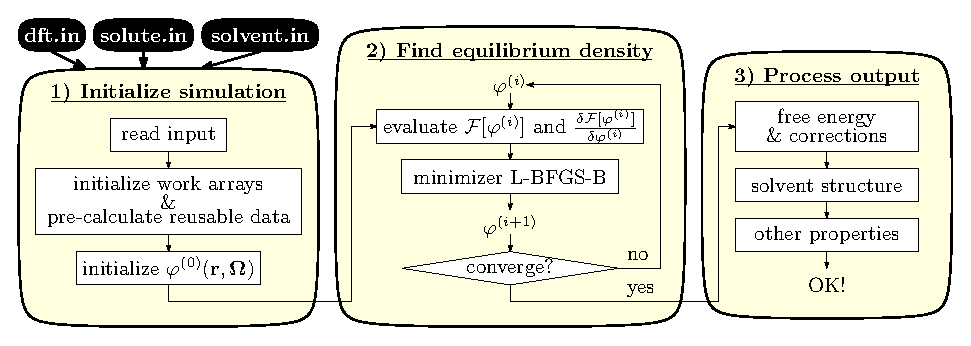
\includegraphics{_figure/mdft}
\par\end{centering}

\caption{Main structure of code MDFT\label{fig:code-mdft}}
\end{figure}



\subsection{Minimizer L-BFGS-B}

The minimizer adopted by MDFT is the L-BFGS-B \citep{Zhu_1994_bfgs,Zhu_bfgs_1997_algorithm}
package version 3.0 written in Fortran 77, implementing the limited-memory
Broyden-Fletcher-Goldfarb-Shanno (BFGS) algorithm with constraints
of the form $l\leq x\leq u$ to the variable $x$. \textcolor{red}{During
the evaluation of the initial code which use L-BFGS,} the constraint
function is not used.

The functional $\mathcal{F}[x_{i}]$ and the gradient of functional
$\nabla\mathcal{F}[x_{i}]=\dfrac{\delta\mathcal{F}}{\delta x}(x_{i})$
are required by L-BFGS to minimize the functional. It saves the variables
$x_{i}$ and gradient of the past $m$ iterations, which is a memory
eater.

The functional in MDFT to be minimized is eq. (\textcolor{red}{ref}),
and its gradient is
\begin{equation}
\frac{\delta\mathcal{F}[\rho]}{\delta\rho(\mathbf{r},\mathbf{\Omega})}=\beta^{-1}\ln\left(\dfrac{\rho(\mathbf{r},\mathbf{\Omega})}{\rho_{0}}\right)+V_{\mathrm{ext}}(\mathbf{r},\mathbf{\Omega})+V_{\mathrm{exc}}(\mathbf{r},\mathbf{\Omega})
\end{equation}
\textcolor{red}{where $\rho_{0}$ is the angular density of bulk solvent
$\rho_{0}=n_{0}/\left(8\pi^{2}\right)$}


\subsection{Treatment to avoid unphysical density}

During minimization, the density variable $\rho(\mathbf{r},\mathbf{\Omega})$
can have an unphysical negative number, \textcolor{red}{which also causes
the divergence of the minimization.} To avoid this phenomenon, a normalized
$\varphi(\mathbf{r},\mathbf{\Omega})$ is used as a variable during
the minimization in place of $\rho(\mathbf{r},\mathbf{\Omega})$,
so that
\begin{equation}
\rho(\mathbf{r},\mathbf{\Omega})=\rho_{0}\varphi^{2}(\mathbf{r},\mathbf{\Omega})\label{eq:cg_vect}
\end{equation}


According to the definition (\ref{eq:cg_vect}), we see
\begin{equation}
\frac{\delta\rho(\mathbf{r},\mathbf{\Omega})}{\delta\varphi}=2\rho_{0}\varphi(\mathbf{r},\mathbf{\Omega})
\end{equation}
Therefore the gradient to feed the L-BFGS minimizer \textcolor{red}{(but
in the code there is additional $\mathrm{d}\mathbf{r}\mathrm{d}\mathbf{\Omega}$
??? for all the three parts)}
\begin{equation}
\frac{\delta\mathcal{F}}{\delta\varphi}=\frac{\delta\mathcal{F}}{\delta\rho}\cdot\frac{\delta\rho}{\delta\varphi}=2\rho_{0}\varphi(\mathbf{r},\mathbf{\Omega})\cdot\left[\beta^{-1}\ln\varphi^{2}+V_{\mathrm{ext}}+V_{\mathrm{exc}}\right]
\end{equation}



\subsection{Evaluation of $V_{\mathrm{ext}}$}

In eq. (\textcolor{red}{ref}) we define the external potential $V_{\mathrm{ext}}$
as the gradient of external free energy functional due to the solute,
or unity \textcolor{red}{{[}{]}}. When the solute is a molecule with a
force field, it contains two components:
\begin{equation}
V_{\mathrm{ext}}(\mathbf{r},\mathbf{\Omega})=V_{\mathrm{LJ}}(\mathbf{r})+V_{\mathrm{coul}}(\mathbf{r},\mathbf{\Omega})
\end{equation}


The Lennard-Jones potential is given by
\begin{equation}
V_{\mathrm{LJ}}(\mathbf{r})=\sum_{u}\sum_{v}4\epsilon_{uv}\left[\left(\dfrac{\sigma_{uv}}{r_{uv}}\right)^{12}-\left(\dfrac{\sigma_{uv}}{r_{uv}}\right)^{6}\right]\label{eq:LJ}
\end{equation}


where $u$ stands for solute,  $v$ stands for solvent, $\epsilon_{uv}=\sqrt{\epsilon_{u}\epsilon_{v}}$
and $\sigma_{uv}=\left(\sigma_{u}+\sigma_{v}\right)$ are the geometric
and arithmetic average Lennard-Jones parameters between solute and
solvent. $r_{ij}$ is the norm of relative site-site vector
\begin{equation}
\mathbf{r}_{uv}=\mathbf{r}+\mathbf{R}(\mathbf{\Omega})\mathbf{s}_{v}-\mathbf{r}_{u}\label{eq:ruv}
\end{equation}
where $\mathbf{r}_{u}$ and $\mathbf{s}_{j}$ are the coordinates
of solute/solvent molecules in the molecular frame, and $\mathbf{R}(\mathbf{\Omega})$ is
the rotation matrix of the Euler angles $\mathbf{\Omega}$.

In cases where the solvent site wears only one LJ centre, eq. (\ref{eq:ruv})
reduces to:

\begin{equation}
\mathbf{r}_{uv}=\mathbf{r}-\mathbf{r}_{u}
\end{equation}
which is exactly what we use in the code as the solvent is SPC/E water.

...

The Coulomb interaction is calculated by \textcolor{red}{solving the
Poisson equation \citep{Marchi_2001}.}

The charge density of the solute is projected onto a space grid,
\begin{equation}
\rho_{q}(\mathbf{r})=\sum_{u}q_{ijk}
\end{equation}
where $q_{ijk}$ is the charge on the space grid distributed by its
nearby point charge as shown in figure \ref{fig:Charge-density-projected}a.

\begin{figure}[h]
\begin{centering}
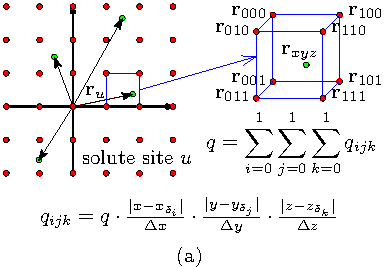
\includegraphics{/Users/lding/Desktop/__M0921/_figure/charge_int}
\par\end{centering}

\caption{Charge density projected onto grids\label{fig:Charge-density-projected}.
(a) Solute. (b) Solvent.}
\end{figure}


\begin{equation}
V_{\mathrm{coul}}(\mathbf{r},\mathbf{\Omega})=\sum_{v}q_{v}V_{q}(\mathbf{r}_{u})
\end{equation}


Poisson solver

Field 
\begin{equation}
E(\mathbf{r})=-\overrightarrow{\nabla}V_{q}(\mathbf{r})
\end{equation}
where $V_{q}(\mathbf{r})$ is ... of unity ...

Local expression of Gauss's theorem 
\begin{equation}
\nabla\cdot E(\mathbf{r})=\frac{\rho_{q}(\mathbf{r})}{\varepsilon_{0}}
\end{equation}
therefore

\begin{equation}
\nabla^{2}V_{q}(\mathbf{r})=-\frac{\rho_{q}(\mathbf{r})}{\varepsilon_{0}}
\end{equation}


\begin{equation}
\hat{V}_{q}(\mathbf{k})=\frac{\hat{\rho}_{q}(\mathbf{k})}{\varepsilon_{0}k^{2}}
\end{equation}
where $\hat{V}_{q}(\mathbf{k})$ is the Fourier transform of $V_{q}(\mathbf{r})$.

The Fourier transform, since the Laplacian is a linear operator:

\begin{eqnarray}
\nabla^{2}f(\mathbf{r}) & = & \nabla^{2}\int\mathrm{d}\mathbf{k}\hat{f}(k)e^{2\pi i\mathbf{r}\cdot\mathbf{k}}\\
 & = & \int\mathrm{d}\mathbf{k}\hat{f}(k)\nabla^{2}e^{2\pi i\mathbf{r}\cdot\mathbf{k}}\\
 & = & \int\mathrm{d}\mathbf{k}\left(-4\pi^{2}\left|\mathbf{k}\right|^{2}\right)\hat{f}(k)e^{2\pi i\mathbf{r}\cdot\mathbf{k}}
\end{eqnarray}


\begin{equation}
\mathcal{F}\left[\nabla^{2}V_{q}(\mathbf{r})\right]=-4\pi^{2}\left|\mathbf{k}\right|^{2}\hat{V}_{q}(\mathbf{k})
\end{equation}
For Fourier series $-4\pi^{2}\left|\mathbf{k}\right|^{2}$ is the
eigenvalue of laplacian:

\begin{equation}
\mathcal{F}\left[\nabla^{2}V_{q}(\mathbf{r})\right]=\mathcal{F}\left[-\frac{\rho_{q}(\mathbf{r})}{\varepsilon_{0}}\right]=\left(i\mathbf{k}\right)^{2}\hat{V}_{q}(\mathbf{k})=-4\pi\hat{\rho}_{q}(\mathbf{k})
\end{equation}


\begin{equation}
\hat{V}_{\mathrm{Poisson}}(\mathbf{k})=\frac{4\pi\hat{\rho}_{q}(\mathbf{k})}{k^{2}}
\end{equation}



\subsection{Evaluation of $V_{\mathrm{exc}}$}

$V_{\mathrm{exc}}$ is ... of unity {[}{]}

Diople

We define $r=\left\Vert \bm{r}-\bm{r}^{\prime}\right\Vert $, and
$\Delta n\left(\bm{r}\right)=n\left(\bm{r}\right)-n_{0}$, and $n_{0}$
the density of the bulk solvent, e.g., 0.0332891 molecule per $\textrm{\AA}^{3}$
for water.

We also define $n\left(\bm{r}\right)=\int\rho(\bm{r},\boldsymbol{\Omega})\mbox{d}\boldsymbol{\Omega}$.
We have 
\begin{eqnarray}
F_{exc} & = & -\frac{1}{2}k_{B}T\iint\Delta n\left(\boldsymbol{r}\right)\Delta n\left(\boldsymbol{r}^{\prime}\right)c\left(r\right)d\bm{r}d\bm{r}^{\prime},
\end{eqnarray}
Now, we consider the convolution in the right-hand side of the equation,
$\gamma\equiv\left(\Delta n*c\right)$, that can be computed much more
efficiently than in $O\left(N^{2}\right)$ by Fast Fourier Transform
in $O\left(N\log N\right)$.

\begin{eqnarray}
\bm{P}\left(\bm{r}\right) & = & \int\bm{p}\rho\left(\bm{r},\bm{\Omega}\right)d\bm{\Omega}
\end{eqnarray}
with $\bm{p}=p\bm{\Omega}$ the dipolar moment of a water molecule.

HRF approximation \citep{Zhao_2011}

Work by Zhao et al.
